% Template PNSAC newsletter - Article
% Language: Latex
%

% Head

\title{Building troop seats for North Star 17515}

\author{Rolf Geiger}

\maketitle



There are no original parts or drawings for the seats. Fortunately,
the tubing and brackets that connect the seats to the aircraft wall
were still in place in the aircraft. Also, two lower tubing support
brackets were found, allowing us to produce exact copies of the
original. Everything else concerning the seats is missing and needs to
be replaced.

\end{multicols}

%\begin{figure*}[htbp]
\begin{figure*}[h]
   \vspace{2em}
   \centering
   %name of the graphic, without the path AND in EPS format:
   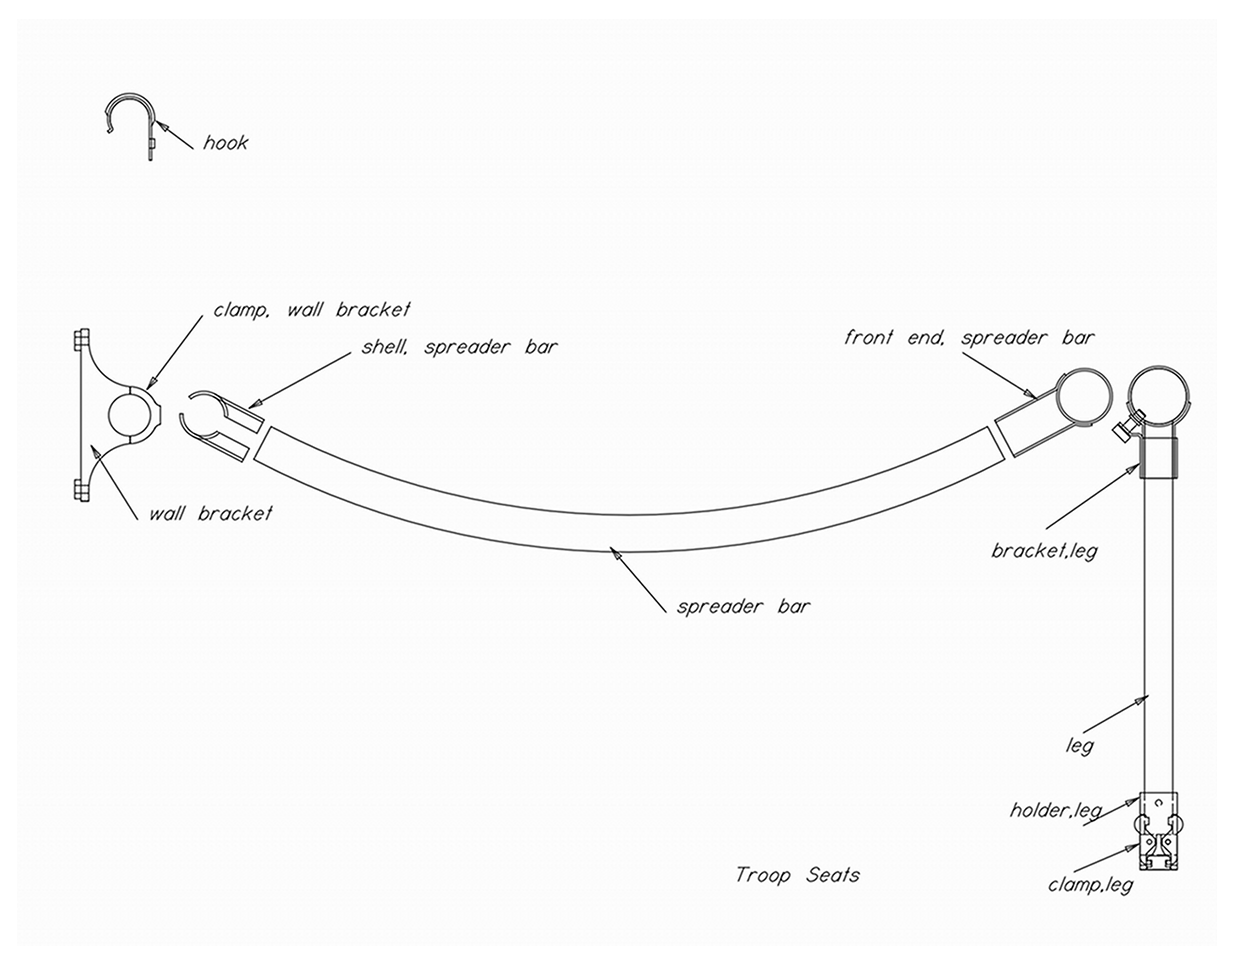
\includegraphics[scale=0.75]{ass.eps}
   %caption of the figure 
   \caption*{\small \em Troop seat construction detail.}
   %label of the figure, which has to correspond to \ref{}:
   \label{fig:ass}
\end{figure*}

\begin{multicols}{2}

To find the size and the number of seats to be produced we measured
the space between the anchoring studs in the aircraft floor, which the
legs snap onto. This gave us the width of the seats. Thus, we will
produce (5) three-seaters plus (6) four-seaters, providing seating for
39 troops. No litters are planned.

Mike Irvin (our Museum coordinator) decided to use seats from a
helicopter in the Museum collection as an example for our seats. We
are more or less copying the parts of these seats, considering that we
have to adapt our methods to the equipment available to us. 

To start the project, drawings of the parts were made. The list of
materials of these parts calls mainly for aluminum bar stock, aluminum
tubing, steel tubing, aluminum sheet and steel sheet. 

\begin{figure}[htbp]
   \vspace{2em}
   \centering
   %name of the graphic, without the path AND in EPS format:
   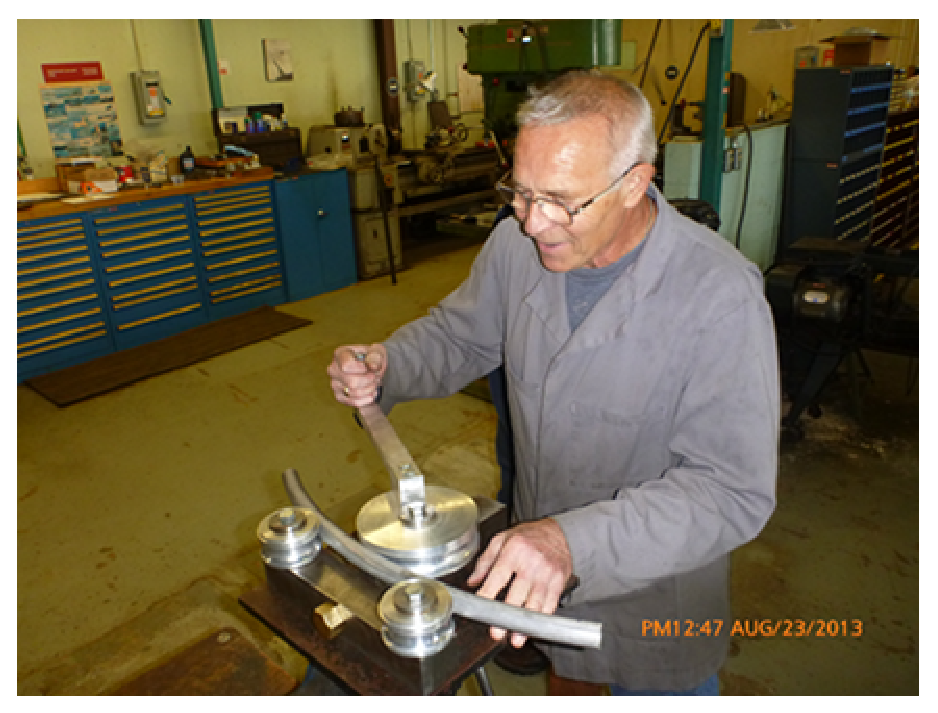
\includegraphics[scale=0.5]{rolf.eps}
   %caption of the figure 
   \caption*{\small \em Rolf Geiger at work on the troop seats.}
   %label of the figure, which has to correspond to \ref{}:
   \label{fig:rolf}
\end{figure}

Thus, we need to produce (15) different metal parts, including: lower
tubing plus support brackets and clamps, spreader bars with two shell
clamps each to clamp onto the lower support tubing plus the front
brackets holding the spreader bars to the frontal support tubes, leg
brackets connecting the legs to the frontal support tubes plus
secondary brackets (slipping over the leg brackets) holding a spring
loaded pin with which the seat fabric will be tautened, legs,
including the lower clamping mechanism fastening the legs to the
floor. Most parts need (22) of each, except the shell clamps for the
spreader bars (44), hooks (117), leg grippers (44).
  
The procedure in the production of these parts is as with any project:
Take the finished product and then work backwards to determine the
production stages.

In the case of a formed sheet metal part a drawing of a flattened
blank is produced by calculating bend radii and adding that to the
straight surfaces (in effect un-bending or stretching the finished
part).  

Experimental operations may be needed to find the shape and dimensions
of the blanks.  Tooling may be needed to produce the formed sheet
metal parts.  The blanks are made by shearing and sawing, according
to the parts drawing.

In the case of a machined part, it is usually produced from bar stock:
Parts are cut to length and subsequently machined as per
drawing. Partial in-between drawings may be necessary to produce the
parts in progressive stages.

To avoid the higher costs associated with surface plating the metal
parts, (as per original parts) we chose painting them instead, which
will be acceptable given the limited use of the finished product.

\begin{footnotesize}
    \raggedleft PNSAC\\
\end{footnotesize}

% End of text.

%%% Local Variables: 
%%% mode: latex
%%% TeX-master: main_document.tex
%%% End: 

